\chapter{栈和队列}


\section{栈} %%%%%%%%%%%%%%%%%%%%%%%%%%%%%%


\subsection{Valid Parentheses} %%%%%%%%%%%%%%%%%%%%%%%%%%%%%%
\label{sec:valid-parentheses}


\subsubsection{描述}
Given a string containing just the characters \code{'(', ')', '\{', '\}', '['} and \code{']'}, determine if the input string is valid.

The brackets must close in the correct order, \code{"()"} and \code{"()[]{}"} are all valid but \code{"(]"} and \code{"([)]"} are not.


\subsubsection{分析}
无


\subsubsection{代码}
\begin{Code}
// LeetCode, Valid Parentheses
// 时间复杂度O(n),空间复杂度O(n)
class Solution {
public:
    bool isValid (string const& s) {
        string left = "([{";
        string right = ")]}";
        stack<char> stk;

        for (auto c : s) {
            if (left.find(c) != string::npos) {
                stk.push (c);
            } else {
                if (stk.empty () || stk.top () != left[right.find (c)])
                    return false;
                else
                    stk.pop ();
            }
        }
        return stk.empty();
    }
};
\end{Code}


\subsubsection{相关题目}
\begindot
\item Generate Parentheses, 见 \S \ref{sec:generate-parentheses}
\item Longest Valid Parentheses, 见 \S \ref{sec:longest-valid-parentheses}
\myenddot


\subsection{Longest Valid Parentheses} %%%%%%%%%%%%%%%%%%%%%%%%%%%%%%
\label{sec:longest-valid-parentheses}


\subsubsection{描述}
Given a string containing just the characters \code{'('} and \code{')'}, find the length of the longest valid (well-formed) parentheses substring.

For \code{"(()"}, the longest valid parentheses substring is \code{"()"}, which has length = 2.

Another example is \code{")()())"}, where the longest valid parentheses substring is \code{"()()"}, which has length = 4.


\subsubsection{分析}
无


\subsubsection{使用栈}
\begin{Code}
// LeetCode, Longest Valid Parenthese
// 使用栈,时间复杂度O(n),空间复杂度O(n)
class Solution {
public:
    int longestValidParentheses(string s) {
        int max_len = 0, last = -1; // the position of the last ')'
        stack<int> lefts;  // keep track of the positions of non-matching '('s

        for (int i = 0; i < s.size(); ++i) {
            if (s[i] =='(') {
                lefts.push(i);
            } else {
                if (lefts.empty()) {
                    // no matching left
                    last = i;
                } else {
                    // find a matching pair
                    lefts.pop();
                    if (lefts.empty()) {
                        max_len = max(max_len, i-last);
                    } else {
                        max_len = max(max_len, i-lefts.top());
                    }
                }
            }
        }
        return max_len;
    }
};
\end{Code}

\subsubsection{Dynamic Programming, One Pass}
\begin{Code}
// LeetCode, Longest Valid Parenthese
// 时间复杂度O(n),空间复杂度O(n)
// @author 一只杰森(http://weibo.com/wjson)
class Solution {
public:
    int longestValidParentheses(string s) {
        vector<int> f(s.size(), 0);
        int ret = 0;
        for (int i = s.size() - 2; i >= 0; --i) {
            int match = i + f[i + 1] + 1;
            // case: "((...))"
            if (s[i] == '(' && match < s.size() && s[match] == ')') {
                f[i] = f[i + 1] + 2;
                // if a valid sequence exist afterwards "((...))()"
                if (match + 1 < s.size()) f[i] += f[match + 1];
            }
            ret = max(ret, f[i]);
        }
        return ret;
    }
};
\end{Code}


\subsubsection{两遍扫描}
\begin{Code}
// LeetCode, Longest Valid Parenthese
// 两遍扫描,时间复杂度O(n),空间复杂度O(1)
// @author 曹鹏(http://weibo.com/cpcs)
class Solution {
public:
    int longestValidParentheses(string s) {
        int answer = 0, depth = 0, start = -1;
        for (int i = 0; i < s.size(); ++i) {
            if (s[i] == '(') {
                ++depth;
            } else {
                --depth;
                if (depth < 0) {
                    start = i;
                    depth = 0;
                } else if (depth == 0) {
                    answer = max(answer, i - start);
                }
            } 
        }

        depth = 0;
        start = s.size();
        for (int i = s.size() - 1; i >= 0; --i) {
            if (s[i] == ')') {
                ++depth;
            } else {
                --depth;
                if (depth < 0) {
                    start = i;
                    depth = 0;
                } else if (depth == 0) {
                    answer = max(answer, start - i);
                }
            } 
        }
        return answer;
    }
};
\end{Code}


\subsubsection{相关题目}
\begindot
\item Valid Parentheses, 见 \S \ref{sec:valid-parentheses}
\item Generate Parentheses, 见 \S \ref{sec:generate-parentheses}
\myenddot


\subsection{Largest Rectangle in Histogram} %%%%%%%%%%%%%%%%%%%%%%%%%%%%%%
\label{sec:largest-rectangle-in-histogram}


\subsubsection{描述}
Given $n$ non-negative integers representing the histogram's bar height where the width of each bar is 1, find the area of largest rectangle in the histogram.

\begin{center}
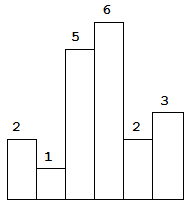
\includegraphics[width=120pt]{histogram.png}\\
\figcaption{Above is a histogram where width of each bar is 1, given height = \fn{[2,1,5,6,2,3]}.}\label{fig:histogram}
\end{center}

\begin{center}
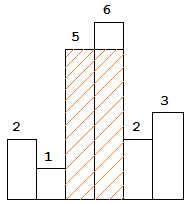
\includegraphics[width=120pt]{histogram-area.png}\\
\figcaption{The largest rectangle is shown in the shaded area, which has area = 10 unit.}\label{fig:histogram-area}
\end{center}

For example,
Given height = \fn{[2,1,5,6,2,3]},
return 10.


\subsubsection{分析}
简单的,类似于 Container With Most Water(\S \ref{sec:container-with-most-water}),对每个柱子,左右扩展,直到碰到比自己矮的,计算这个矩形的面积,用一个变量记录最大的面积,复杂度$O(n^2)$,会超时。

如图\S \ref{fig:histogram-area}所示,从左到右处理直方,当$i=4$时,小于当前栈顶(即直方3),对于直方3,无论后面还是前面的直方,都不可能得到比目前栈顶元素更高的高度了,处理掉直方3(计算从直方3到直方4之间的矩形的面积,然后从栈里弹出);对于直方2也是如此;直到碰到比直方4更矮的直方1。

这就意味着,可以维护一个递增的栈,每次比较栈顶与当前元素。如果当前元素大于栈顶元素,则入栈,否则合并现有栈,直至栈顶元素小于当前元素。结尾时入栈元素0,重复合并一次。


\subsubsection{代码}
\begin{Code}
// LeetCode, Largest Rectangle in Histogram
// 时间复杂度O(n),空间复杂度O(n)
class Solution {
public:
    int largestRectangleArea(vector<int> &height) {
        stack<int> s;
        height.push_back(0);
        int result = 0;
        for (int i = 0; i < height.size(); ) {
            if (s.empty() || height[i] > height[s.top()])
                s.push(i++);
            else {
                int tmp = s.top();
                s.pop();
                result = max(result,
                        height[tmp] * (s.empty() ? i : i - s.top() - 1));
            }
        }
        return result;
    }
};
\end{Code}


\subsubsection{相关题目}
\begindot
\item Trapping Rain Water, 见 \S \ref{sec:trapping-rain-water}
\item Container With Most Water, 见 \S \ref{sec:container-with-most-water}
\myenddot


\subsection{Evaluate Reverse Polish Notation} %%%%%%%%%%%%%%%%%%%%%%%%%%%%%%
\label{sec:Evaluate-Reverse-Polish-Notation}


\subsubsection{描述}
Evaluate the value of an arithmetic expression in Reverse Polish Notation.

Valid operators are \fn{+, -, *, /}. Each operand may be an integer or another expression.

Some examples:
\begin{Code}
  ["2", "1", "+", "3", "*"] -> ((2 + 1) * 3) -> 9
  ["4", "13", "5", "/", "+"] -> (4 + (13 / 5)) -> 6
\end{Code}


\subsubsection{分析}
无


\subsubsection{递归版}
\begin{Code}
// LeetCode, Evaluate Reverse Polish Notation
// 递归,时间复杂度O(n),空间复杂度O(logn)
class Solution {
public:
    int evalRPN(vector<string> &tokens) {
        int x, y;
        auto token = tokens.back();  tokens.pop_back();
        if (is_operator(token))  {
            y = evalRPN(tokens);
            x = evalRPN(tokens);
            if (token[0] == '+')       x += y;
            else if (token[0] == '-')  x -= y;
            else if (token[0] == '*')  x *= y;
            else                       x /= y;
        } else  {
            size_t i;
            x = stoi(token, &i);
        }
        return x;
    }
private:
    bool is_operator(const string &op) {
        return op.size() == 1 && string("+-*/").find(op) != string::npos;
    }
};
\end{Code}


\subsubsection{迭代版}
\begin{Code}
// LeetCode, Max Points on a Line
// 迭代,时间复杂度O(n),空间复杂度O(logn)
class Solution {
public:
    int evalRPN(vector<string> &tokens) {
        stack<string> s;
        for (auto token : tokens) {
            if (!is_operator(token)) {
                s.push(token);
            } else {
                int y = stoi(s.top());
                s.pop();
                int x = stoi(s.top());
                s.pop();
                if (token[0] == '+')       x += y;
                else if (token[0] == '-')  x -= y;
                else if (token[0] == '*')  x *= y;
                else                       x /= y;
                s.push(to_string(x));
            }
        }
        return stoi(s.top());
    }
private:
    bool is_operator(const string &op) {
        return op.size() == 1 && string("+-*/").find(op) != string::npos;
    }
};
\end{Code}


\subsubsection{相关题目}
\begindot
\item 无
\myenddot


\section{队列} %%%%%%%%%%%%%%%%%%%%%%%%%%%%%%

